\documentclass{standalone}

\usepackage[OT1]{fontenc}
\renewcommand*\familydefault{\sfdefault}
\usepackage{helvet,sfmath}
\usepackage{siunitx}

\usepackage{tikz}
\usetikzlibrary{arrows,calc,patterns}
% \usetikzlibrary{intersections, calc, arrows.meta}
\usepackage{tikz,tkz-euclide}

\begin{document}

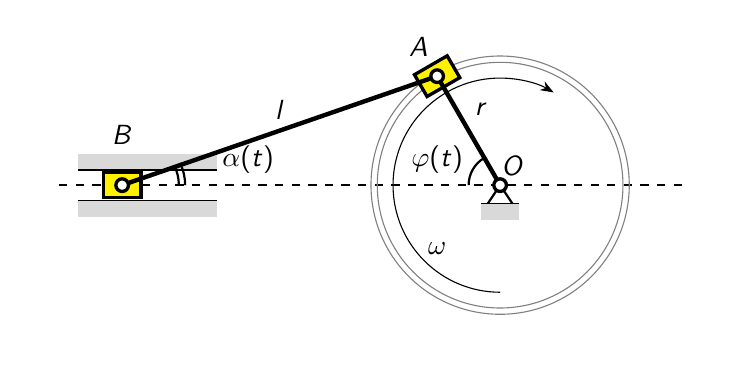
\begin{tikzpicture}[scale=0.8]
    %%Background
    \draw[draw=none] (-0.5,-2.5) rectangle (10.5,2.5);
    %%
    \draw[thick, dashed] (0,0) to (10,0);
    \draw[gray] (7,0) circle (1.95);
    \draw[gray] (7,0) circle (2.05);

    \draw[thick] (0.3,0.25) to (2.5,0.25);
    \draw[thick] (0.3,-0.25) to (2.5,-0.25);
    \draw[draw=none, fill = gray!30] (0.3,0.25) rectangle (2.5,0.5);
    \draw[draw=none, fill = gray!30] (0.3,-0.25) rectangle (2.5,-0.5);

    \draw[thick] (7,0) to (7.2,-0.3);
    \draw[thick] (7,0) to (6.8,-0.3);
    \draw[thick] (6.7,-0.3) to (7.3,-0.3);
    \draw[draw=none, fill = gray!30] (6.7,-0.3) rectangle (7.3,-0.55);
    

    \draw[fill=yellow, very thick] (0.7,-0.2) rectangle (1.3,0.2);
    \begin{scope}[rotate around={30:(6,1.73)}]
        \draw[fill=yellow, very thick] (5.7,1.53) rectangle (6.3,1.93);
    \end{scope}
    
    \draw[ultra thick] (7,0) to (6,1.73) to (1,0);
    \filldraw[color=black, fill=white, very thick] (1,0) circle (0.1);
    \filldraw[color=black, fill=white, very thick](6,1.73) circle (0.1);
    \filldraw[color=black, fill=white, very thick](7,0) circle (0.1);

    \draw[thick] (6.5,0) arc (180:120:0.5);
    \draw[thick] (1.9,0) arc (0:27:0.7);
    \draw[thick] (2,0) arc (0:26:0.8);

    \draw[-Stealth] (7,-1.7) arc(270:60:1.7);

    \draw
    (3.5,1.2) node{\(l\)}
    (6.7,1.2) node{\(r\)}
    (6,0.4) node{\(\varphi (t)\)}
    (3,0.4) node{\(\alpha (t)\)}
    (7.2,0.3) node{\(O\)}
    (5.7,2.2) node{\(A\)}
    (1,0.8) node{\(B\)}
    (6,-1) node{\(\omega\)}
    ;
    
\end{tikzpicture}

\end{document}
